\documentclass[aspectratio=169]{../latex_main/tntbeamer}  % you can pass all options of the beamer class, e.g., 'handout' or 'aspectratio=43'
\usepackage{dsfont}
\usepackage{bm}
\usepackage[english]{babel}
\usepackage[T1]{fontenc}
%\usepackage[utf8]{inputenc}
\usepackage{graphicx}
\graphicspath{ {./figures/} }
\usepackage{algorithm}
\usepackage[ruled,vlined,algo2e,linesnumbered]{algorithm2e}
\usepackage{hyperref}
\usepackage{booktabs}
\usepackage{mathtools}

\usepackage{amsmath,amssymb}

\DeclareMathOperator*{\argmax}{arg\,max}
\DeclareMathOperator*{\argmin}{arg\,min}

\usepackage{pgfplots}
\pgfplotsset{compat=1.16}
\usepackage{tikz}
\usetikzlibrary{trees} 
\usetikzlibrary{shapes.geometric}
\usetikzlibrary{positioning,shapes,shadows,arrows,calc,mindmap}
\usetikzlibrary{positioning,fadings,through}
\usetikzlibrary{decorations.pathreplacing}
\usetikzlibrary{intersections}
\pgfdeclarelayer{background}
\pgfdeclarelayer{foreground}
\pgfsetlayers{background,main,foreground}
\tikzstyle{activity}=[rectangle, draw=black, rounded corners, text centered, text width=8em]
\tikzstyle{data}=[rectangle, draw=black, text centered, text width=8em]
\tikzstyle{myarrow}=[->, thick, draw=black]

% Define the layers to draw the diagram
\pgfdeclarelayer{background}
\pgfdeclarelayer{foreground}
\pgfsetlayers{background,main,foreground}

% Requires XeLaTeX or LuaLaTeX
\usepackage{unicode-math}

\usepackage{fontspec}
%\setsansfont{Arial}
\setsansfont{RotisSansSerifStd}[ 
Path=../latex_main/fonts/,
Extension = .otf,
UprightFont = *-Regular,  % or *-Light
BoldFont = *-ExtraBold,  % or *-Bold
ItalicFont = *-Italic
]
\setmonofont{Cascadia Mono}[
Scale=0.8
]

% scale factor adapted; mathrm font added (Benjamin Spitschan @TNT, 2021-06-01)
%\setmathfont[Scale=1.05]{Libertinus Math}
%\setmathrm[Scale=1.05]{Libertinus Math}

% other available math fonts are (not exhaustive)
% Latin Modern Math
% XITS Math
% Libertinus Math
% Asana Math
% Fira Math
% TeX Gyre Pagella Math
% TeX Gyre Bonum Math
% TeX Gyre Schola Math
% TeX Gyre Termes Math

% Literature References
\newcommand{\lit}[2]{\href{#2}{\footnotesize\color{black!60}[#1]}}

%%% Beamer Customization
%----------------------------------------------------------------------
% (Don't) Show sections in frame header. Options: 'sections', 'sections light', empty
\setbeamertemplate{headline}{empty}

% Add header logo for normal frames
\setheaderimage{
	% 
\includegraphics[height=\logoheight]{figures/TNT_darkv4.pdf}
	
\includegraphics[height=\logoheight]{../latex_main/figures/luh_logo_rgb_0_80_155.pdf}
	% 
\includegraphics[height=\logoheight]{figures/logo_tntluh.pdf}
}

% Header logo for title page
\settitleheaderimage{
	% 
\includegraphics[height=\logoheight]{figures/TNT_darkv4.pdf}
	
\includegraphics[height=\logoheight]{../latex_main/figures/luh_logo_rgb_0_80_155.pdf}
	% 
\includegraphics[height=\logoheight]{figures/logo_tntluh.pdf}
}

% Title page: tntdefault 
\setbeamertemplate{title page}[tntdefault]  % or luhstyle
% Add optional title image here
%\addtitlepageimagedefault{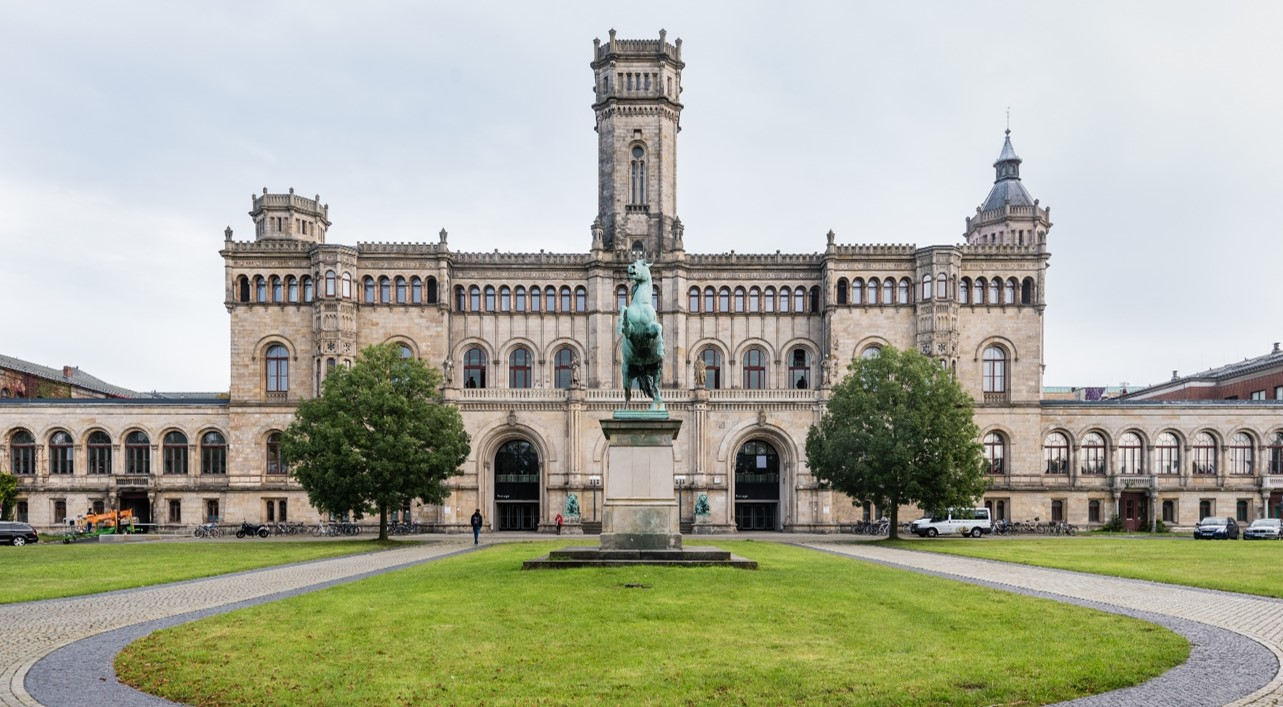
\includegraphics[width=0.65\textwidth]{figures/luh_default_presentation_title_image.jpg}}

% Title page: luhstyle
% \setbeamertemplate{title page}[luhstyle]
% % Add optional title image here
% \addtitlepageimage{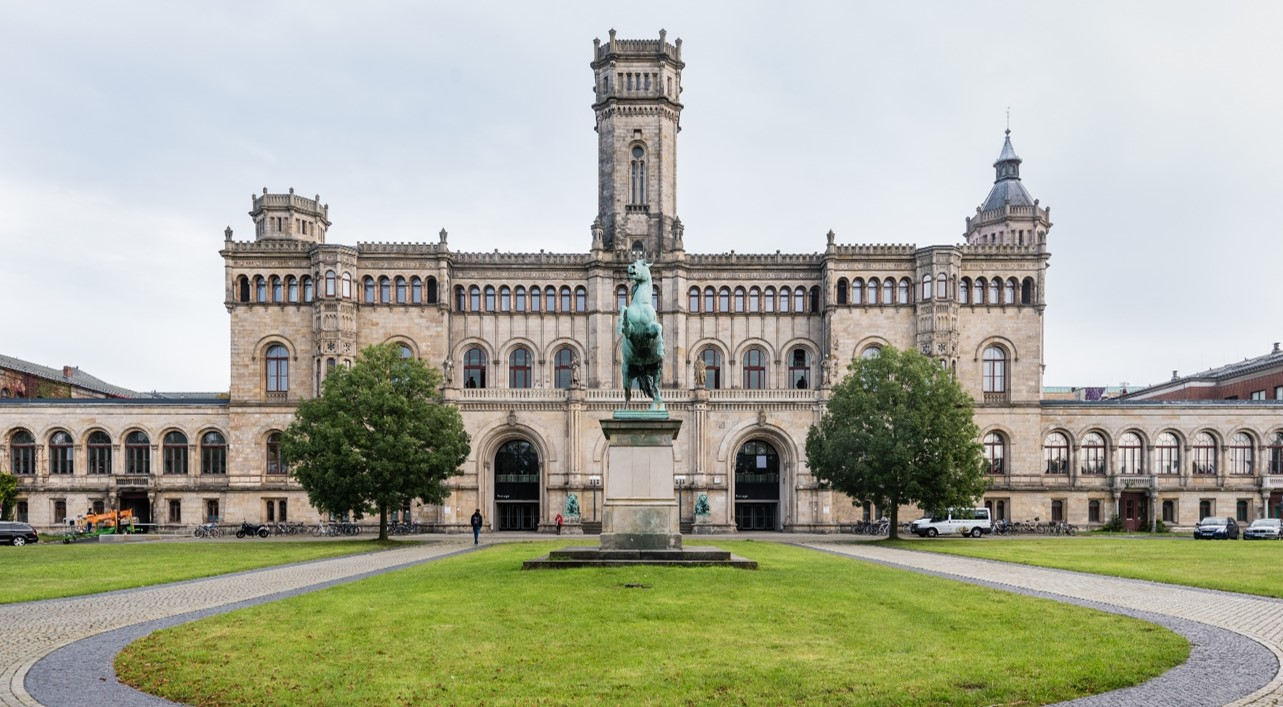
\includegraphics[width=0.75\textwidth]{figures/luh_default_presentation_title_image.jpg}}

\author[Lindauer \& Anand]{Marius Lindauer and Avishek Anand\\[1em]
	
\includegraphics[height=\logoheight]{../latex_main/figures/luh_logo_rgb_0_80_155.pdf}\qquad

\includegraphics[height=\logoheight]{../latex_main/figures/TNT_darkv4}\qquad

\includegraphics[height=\logoheight]{../latex_main/figures/L3S.jpg}	}
\date{Winter Term 2021
}


%%% Custom Packages
%----------------------------------------------------------------------
% Create dummy content
\usepackage{blindtext}

% Adds a frame with the current page layout. Just call \layout inside of a frame.
\usepackage{layout}


\title[Introduction]{iML: Introduction}
\subtitle{Logistics for the Lecture}

%\institute{}


\begin{document}
	
	\maketitle

%-----------------------------------------------------------------------------------------------------------------------------
\begin{frame}[c]{Acknowledgments}

Large parts of the material (i.e. slides and figures) in the first to fifth weeks of the lecture were created by \lit{Bernd Bischl, Giuseppe Casalicchio et al.}{https://www.slds.stat.uni-muenchen.de}. We thank them very much for allowing us to re-use their material.


\end{frame}
%-----------------------------------------------------------------------


%-----------------------------------------------------------------------------------------------------------------------------
\begin{frame}[c]{Goals of the Lecture}

You will be able to \ldots
\begin{enumerate}
  \item \alert{identify} cases where interpreting machine learning models is important
  \item \alert{choose} an appropriate technique for an iML task at hand
  \item \alert{evaluate} the pros and cons of different iML approaches
  \item \alert{apply} iML approaches to a task at hand
\end{enumerate}

\end{frame}
%-----------------------------------------------------------------------
%----------------------------------------------------------------------
\begin{frame}[c]{Course Overview}

\begin{itemize}
	\item Introduction \& Background 
	\item GAMs and Rule-based approaches 
	\item Feature Effects
	\item Local Explanations
	\item Shapley Values for Explainability
	\item Instance-wise Feature Selection
	\item Gradient based Feature attribution
	\item Actionable Explanation and Recourse
	\item Evaluating Interpretability and Utility
	\item Conclusions 
\end{itemize}


\end{frame}
%----------------------------------------------------------------------
%----------------------------------------------------------------------
\begin{frame}[c]{Course Format}

\begin{itemize}
	\item Concepts over details
	\begin{itemize}
	  \item we provide references and links to papers\\ s.t. you can read up details!
	\end{itemize}
	\smallskip
	\item Interactive lecture
	\begin{itemize}
	  \item more efficient learning through self-reflection
	\end{itemize}
	\smallskip
	\item Practical exercises and projects
	\begin{itemize}
	  \item implement it, use it and play with it!
	\end{itemize}
\end{itemize}

\end{frame}
%----------------------------------------------------------------------
%----------------------------------------------------------------------
\begin{frame}[c]{Team}

\begin{columns}[T]

\column{0.2\textwidth}
\centering
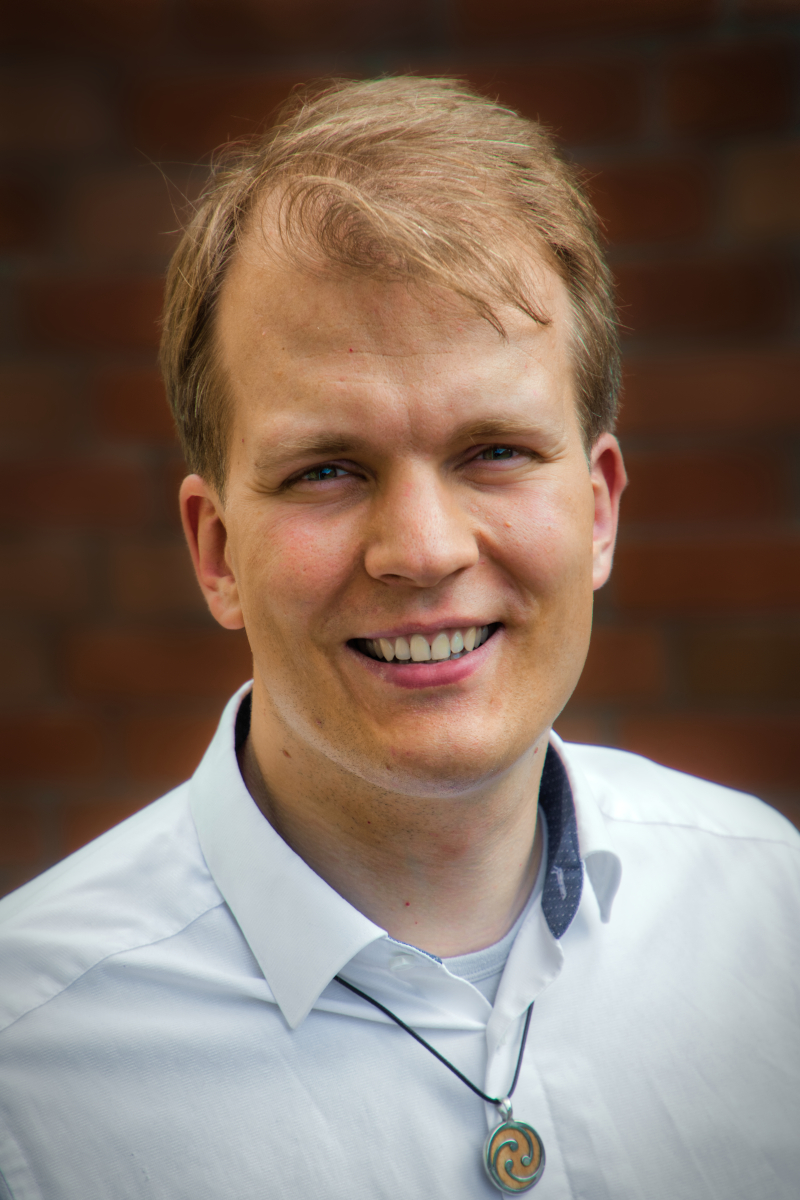
\includegraphics[height=10em]{./figures/marius_lindauer_small}

Prof. Dr.\\ Marius Lindauer

\column{0.2\textwidth}
\centering
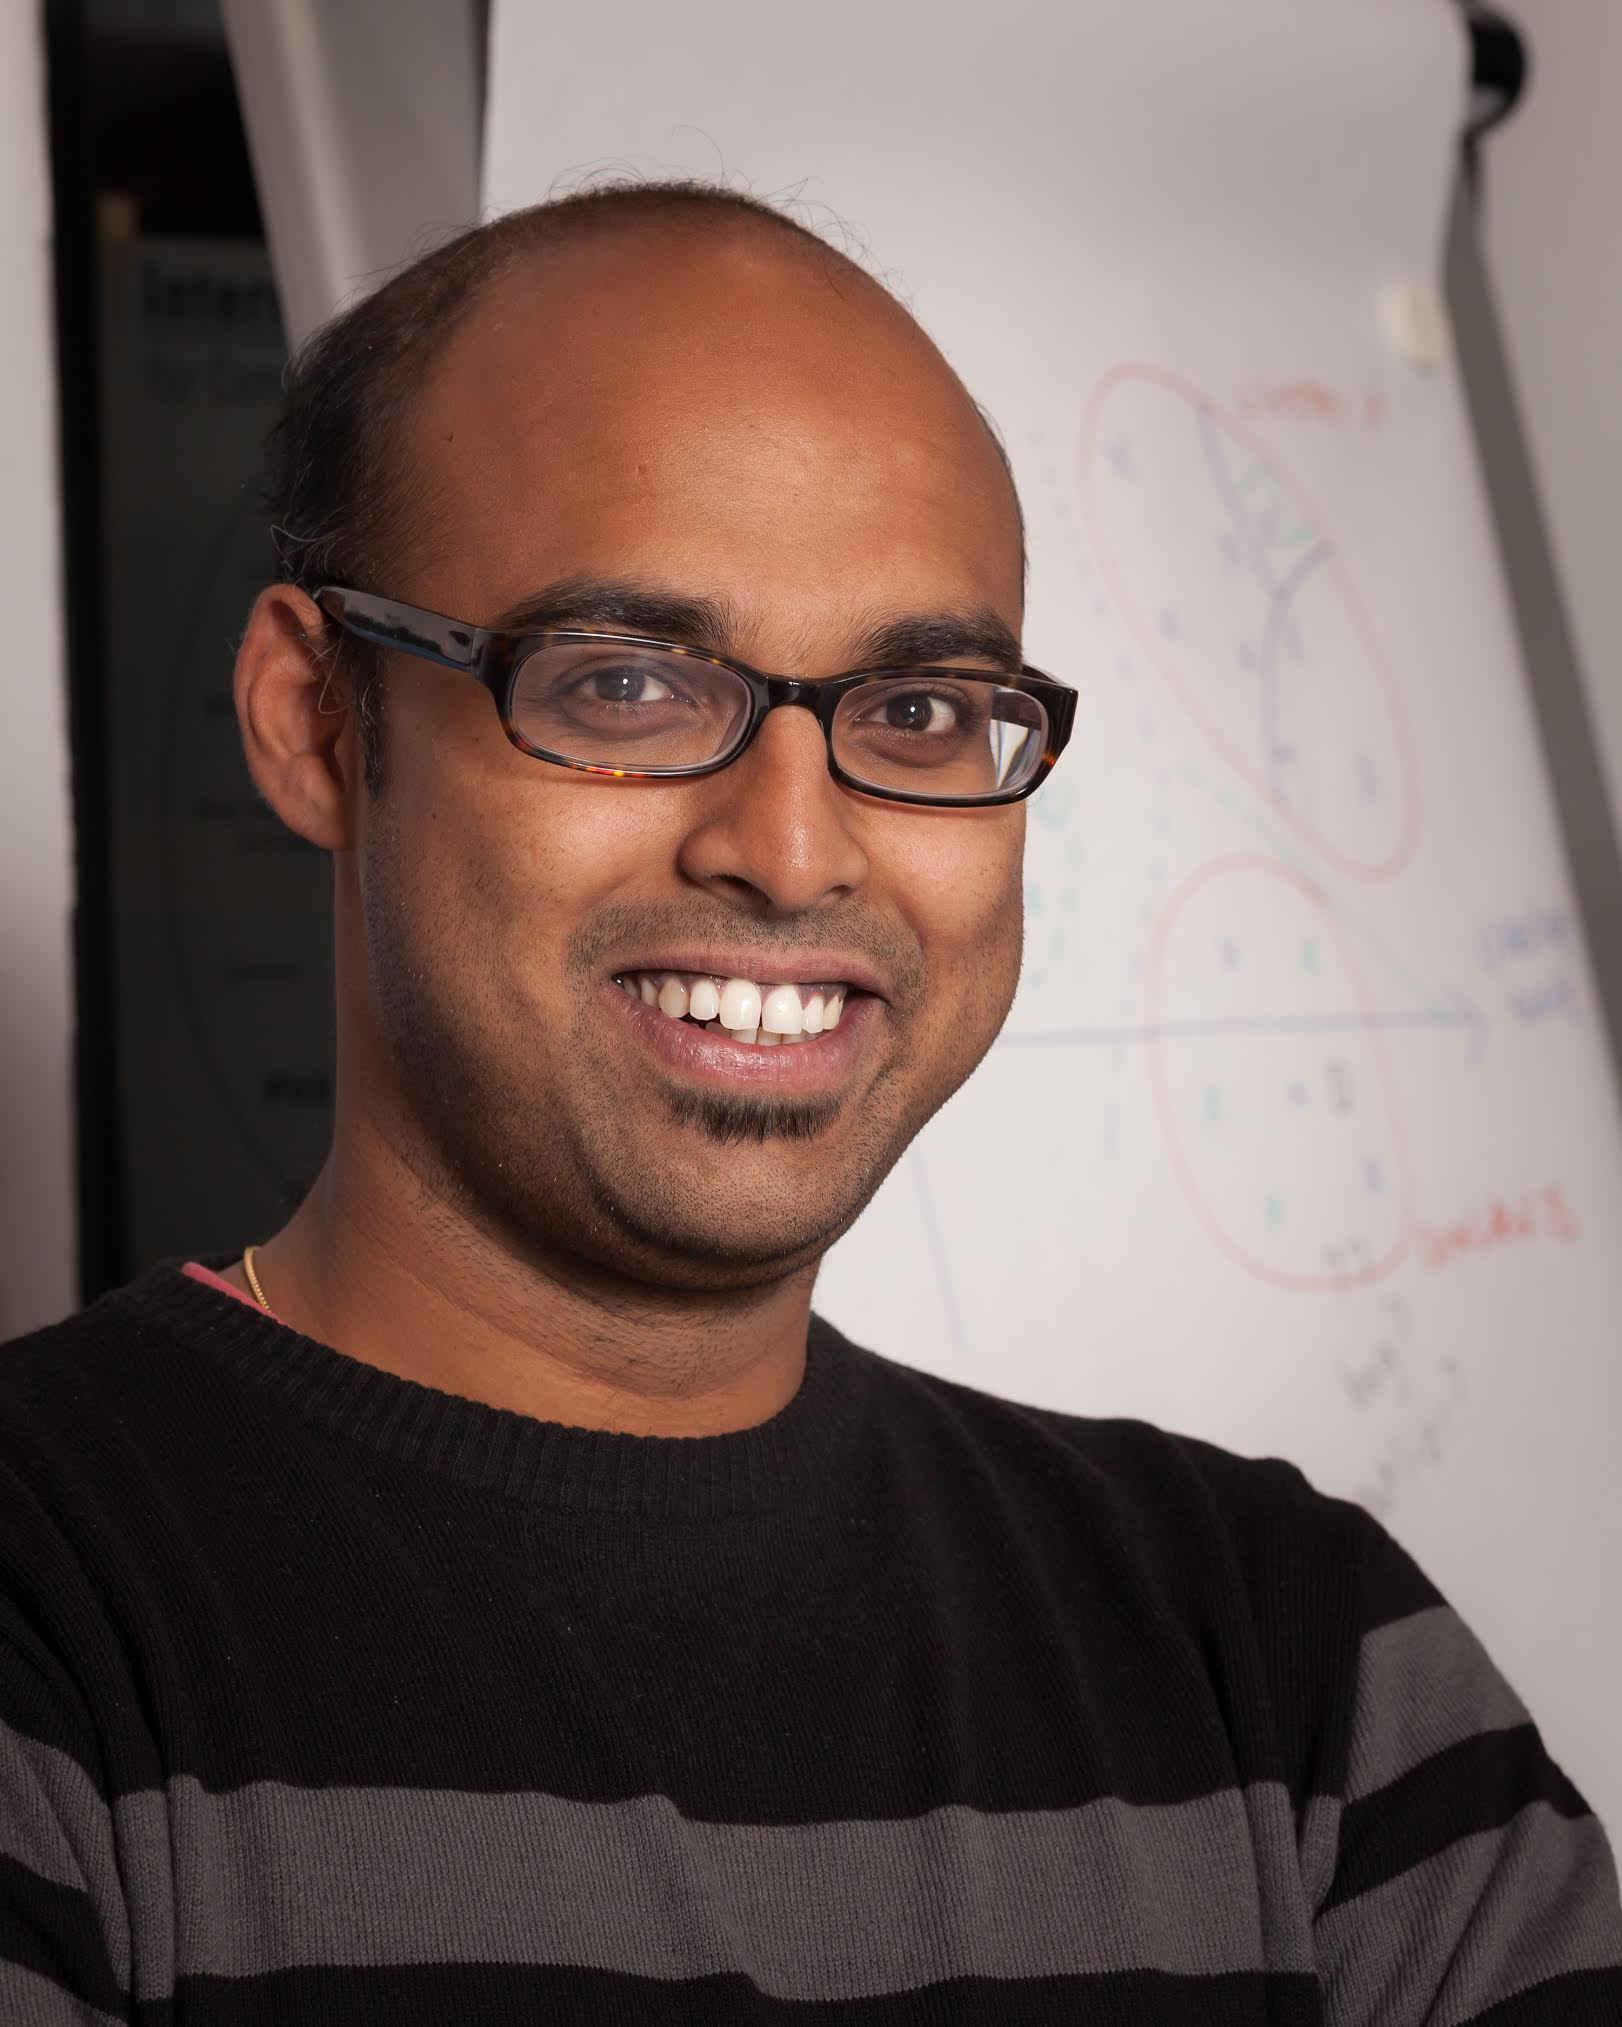
\includegraphics[height=10em]{./figures/avishek-homepage}

Prof. Dr.\\ Avishek Anand

\column{0.2\textwidth}
\centering
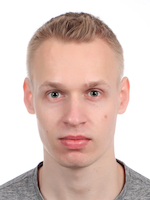
\includegraphics[height=10em]{./figures/rene_sass}

Ren\'e Sass\\

\column{0.2\textwidth}
\centering
\includegraphics[height=10em]{images/TODO.jpg}

??? ???\\

\end{columns}

\end{frame}
%----------------------------------------------------------------------
%----------------------------------------------------------------------
\begin{frame}[c]{Why Videos?}

\begin{itemize}
  \item Advantages of videos:
  \begin{itemize}
      \item Watch it whenever (wherever) you want
      \item Watch it at your own speed
      \begin{itemize}
          \item[$\leadsto$] Stop it if you need time to think about it
      \end{itemize}
      \item Go back and watch it again, if you missed or forgot something
      \item Annotate questions on the fly %(e.g., using the Miro boards)
      \item After each video ($\sim$10-20min), you can take a break and\\ think about what you learned in this video (and whether you understood it)
  \end{itemize}
  \medskip
  \pause
  \item Risks and challenges:
  \begin{itemize}
      \item You have to be self-disciplined 
      \item You have to wait with your questions until our meetings
      \begin{itemize}
          \item[$\leadsto$] Use our chat to discuss with your peers
      \end{itemize}
  \end{itemize}
\end{itemize}

\end{frame}
%-----------------------------------------------------------------------
%----------------------------------------------------------------------
\begin{frame}[c]{Organization (Exercises)}

\begin{itemize}
  \item Every week new exercise sheet
  \begin{itemize}
      \item Exercise focus is aligned with videos
      \item Watch videos and start to directly work on exercise 
      \item[$\leadsto$] \alert{Deadline one day after the live session: Wednesday at 23:59}
  \end{itemize}
  \item Most exercises will be practical, i.e., you have to implement something
  \begin{itemize}
    \item Expected work load: 1.5h - 2h each week
  \end{itemize}
  \item Team work highly recommended, team size at most 3! 
  \item Build upon GitHub classroom $\leadsto$ enables auto-grading
  \begin{itemize}
      \item There will be an invitation link each week -- distributed via Mattermost
  \end{itemize}
%   \item Submit solutions via git
  \pause
  \item Don't cheat (incl. plagiarism)
  \begin{itemize}
    \item First time cheating: $0$ points for exercise
    \item Second time cheating: failing the course
  \end{itemize}
  \pause
  \item Exercises are not mandatory\\ \alert{BUT: quite unlikely that you will pass the course without doing them}
  \pause
  \item Up to \alert{$25$ bonus points} for final grade.
\end{itemize}

\end{frame}
%-----------------------------------------------------------------------
%----------------------------------------------------------------------
\begin{frame}[c]{Live Discussion}

\begin{itemize}
  \item Every week at Tuesday: 09:30am (s.t) - 11:30am\\ 
  \item Room: MRR at L3S (if COVID allows it)
  \pause
  \item Warning: Does not replace watching the recorded lecture videos!
  \pause
  \smallskip
  \item Components:
  \begin{enumerate}
       \item You can ask anything related to the recent lecture videos or exercises
      \item Break-out rooms to discuss questions in small groups
      \pause
      \item Q\&A regarding the exercise
      \pause
      \item Interactive quiz where you can check whether you understood the main points
  \end{enumerate}
  \pause
  \medskip
  \item No recordings of the live sessions (regardless whether virtual or on-site)
\end{itemize}

\end{frame}
%-----------------------------------------------------------------------
%----------------------------------------------------------------------
\begin{frame}[c]{Get in Touch with Us}

\begin{itemize}
  \item Live session every Tuesday (09:30am s.t.)
%   \item Mattermost Chat:
%   \begin{itemize}
%       \item \alert{Use your real names}
%       \item \url{LINK}
%       \item First use the channel "2021/22 iML Lecture"
%       \item Contact us individually only if these are personal questions\\ (such as ``I'm sick and have to cancel my exam'')
%   \end{itemize}
  \item Use the forum in StudIP for all kind of questions
  \item Don't send us emails
  \begin{itemize}
      \item[$\leadsto$] Only in case of emergencies (and even in such cases it is better to use Mattermost) 
  \end{itemize}
\end{itemize}

\end{frame}
%-----------------------------------------------------------------------
%----------------------------------------------------------------------
\begin{frame}[c]{Requirements for Attending}

\begin{itemize}
  \item Knowledge and hands-on exp. in \alert{Machine Learning}\\ (mandatory)
  \begin{itemize}
    \item Classification, regression, clustering, decision tree, training-test split, cross validation, pre-processing \ldots
    \item as offered by Prof. Rosenhahn
    \item to catch up (if nec.): \url{https://www.coursera.org/learn/machine-learning} 
  \end{itemize}
  \pause
  \item Knowledge and hands-on exp. in \alert{Deep Learning} (PyTorch)\\ (mandatory)
  \begin{itemize}
    \item feed-forward network, recurrent network, convolutions, learning rates, regularization, \ldots 
    \item as offered by Prof. Anand
    \item to catch up (if nec.): \url{https://course.fast.ai/}
  \end{itemize}
  \pause
  \item Experience in \alert{Python and git}\\ (mandatory)
  \begin{itemize}
    \item all exercises will require 
    that you implement something in~Python and\\ submit the solution to a git repo
  \end{itemize}
\end{itemize}

\end{frame}
%-----------------------------------------------------------------------
%----------------------------------------------------------------------
\begin{frame}[c]{Final Oral/Project Exam -- Tentative Plan!}

\begin{itemize}
  \item Implement a larger project (worth $1-2$ weeks full time)
  \begin{itemize}
 		\item We will propose topics, where you can choose from
 		\item Team work with up to $3$ students possible
  \end{itemize}
  \pause
  \item Exam
	\begin{itemize}
		\item Present the project in the first $15$ minutes
		\item Q\&A for at most another $15$ minutes
		    \begin{itemize}
		        \item could also be related to other topics of the course, \\
		        e.g., how does your approach relates to XYZ?
		    \end{itemize}
	\end{itemize}	
  \item Tentative date: March DAY1th - DAYENDth
  \pause
  \item If the COVID-19 situation has not improved by then, we will offer virtual oral exams 
  \begin{itemize}
      \item[$\leadsto$] webcam and stable internet connection required!
  \end{itemize}
\end{itemize}

\end{frame}
%----------------------------------------------------------------------
%----------------------------------------------------------------------
\begin{frame}[c]{Additional Resources}

\begin{itemize}
  \item To get a deep understanding of iML,\\ you should also read some papers 
  \item We provide links to important papers after each video
  \item iML books: 
  \begin{itemize}
      \item \url{https://christophm.github.io/interpretable-ml-book/}
      \item \url{https://compstat-lmu.github.io/iml_methods_limitations/}
      \item \url{https://ema.drwhy.ai/}
  \end{itemize}
\end{itemize}

\end{frame}
%----------------------------------------------------------------------
%----------------------------------------------------------------------
\begin{frame}[c]{Opportunities and Risks}

iML is an advanced lecture and we update it each time.

\bigskip
\pause

Opportunities:
\begin{itemize}
  \item All presented topics (except some basics) are close to state-of-the-art;\\there is active research on these topics  
  \item The course will provide a solid background\\ for doing a master project/thesis in our group 
\end{itemize}

\medskip

Risks:
\begin{itemize}
  \item You will find some typos and issues in the slides;\\ please tell us if you find something
\end{itemize}

\medskip
$\to$ Give us some feedback and we will improve the course!


\end{frame}
%-----------------------------------------------------------------------
%----------------------------------------------------------------------
\begin{frame}[c]{Additional Bonus Points}

\begin{itemize}
    \item GitHub repos:
    \begin{itemize}
        \item Slides: \url{https://github.com/automl-edu/iML_lecture}
      %  \item Exercises: \url{???}
    \end{itemize}
    \item If you find bugs in the slides or exercises,\\ students from Hannover can obtain bonus points:
    \begin{itemize}
        \item 1 point for every major bug in an equation
        \item 0.5 point for every typo in the slides
        \item 1 point for every code bug in the exercise
    \end{itemize}
    \item At most 10 points 
    \item Submit a PR to our repos and ensure that we can decipher your real name
    \medskip
    \item Overall, you cannot obtain more than $25$ bonus points from exercise + these
\end{itemize}


\end{frame}
%-----------------------------------------------------------------------
%----------------------------------------------------------------------
\begin{frame}[c]{ToDos for Next Week}


\begin{enumerate}
    \item Watch the videos of the \alert{1st week}
    \item Work on the first exercise sheet
\end{enumerate}

\end{frame}
%-----------------------------------------------------------------------

% \end{frame}

\begin{frame}[c]{}

\centering
\huge
Questions?

\end{frame}

	
\end{document}
